\documentclass[11pt,fleqn]{exam}
\usepackage[utf8]{inputenc}

\usepackage[margin=1in]{geometry}
\usepackage{amsmath,amssymb}
\usepackage{gensymb}
\usepackage{multicol}
\usepackage{float}
\usepackage{graphicx}
\usepackage{units,icomma}
\usepackage[colorlinks,linkcolor=blue,urlcolor=blue]{hyperref}
\usepackage[margin=1.5cm]{caption}

\hyphenation{
  chro-no-ampe-ro-met-ric
  ber-dia-me-ter
  de-ngan
  me-nem-pati
  mic-ro-graphs}

\renewcommand{\figurename}{Gambar.}
\def\equationautorefname{Persamaan}
\newcommand{\class}{OLIMPIADE ASTRONOMI}
\newcommand{\term}{Tingkat Kabupaten/Kota - 2017}
\newcommand{\examnum}{OSK Astronomi 2017}
%\newcommand{\examdate}{11/02/2014}
%\newcommand{\timelimit}{120 Minutes}

\pagestyle{head}
\firstpageheader{}{}{}
\runningheader{\examnum}{}{Halaman \thepage\ dari \numpages}
\runningheadrule


\begin{document}

\noindent
\begin{tabular*}{\textwidth}{l @{\extracolsep{\fill}} r @{\extracolsep{6pt}} l}
\textbf{\class} \\% & \textbf{Name:} & \makebox[2in]{\hrulefill}\\
\textbf{\term}  %&&\\
%\textbf{\examnum} &&\\
%\textbf{\examdate} &&\\
%\textbf{Time Limit: \timelimit} & Teaching Assistant & \makebox[2in]{\hrulefill}
\end{tabular*}\\
\rule[2ex]{\textwidth}{2pt}

\noindent
\begin{tabular}{ll}
Copyright (c) 2017 & Ridlo W. Wibowo (ridlo.w.wibowo@gmail.com)\\
                   & Sulistiyowati (sulis.astro08@gmail.com)
\end{tabular}

\vspace{0.3cm}
\noindent
Solusi ini dibuat tanpa jaminan kesesuaian dengan solusi resmi dari juri olimpiade sains bidang Astronomi. Pengguna boleh menyebarluaskan dan/atau memodifikasi solusi ini dengan mencantumkan sumber asli. Hak cipta soal ada pada Kemendiknas dan dilindungi undang-undang.

\vspace{0.4cm}
\noindent
\rule[2ex]{\textwidth}{1.5pt}

\textbf{PILIHAN GANDA (3 POIN PER SOAL)}

\begin{questions}
\question Pada suatu saat, posisi Bumi berada di antara Matahari dan sebuah asteroid. Posisi ketiganya membentuk satu garis lurus. Pada saat tersebut, asteroid tidak terkena bayangan umbra Bumi. Jika jarak Bumi\---Matahari saat itu adalah 1 sa, maka jarak asteroid tersebut dari Bumi harus lebih besar dari
\begin{choices}
\choice $7,68\times 10^{-3}$ sa
\choice $9,25\times 10^5$ km
\choice $5,22\times 10^{-3}$ sa
\choice $1,38\times 10^6$ km
\choice $3,59\times 10^{-3}$ sa
\end{choices}

\textit{Jawaban: D}\\

Karena ketiganya dalam posisi garis lurus, maka jarak asteroid harus lebih besar dari panjang umbra bumi ($d_{\text{umbra}}$).

\begin{figure}[!ht]
\centering
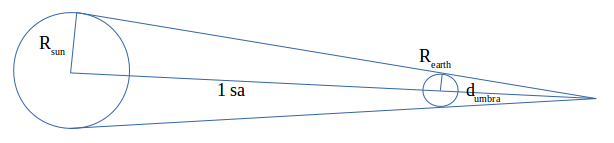
\includegraphics[width=0.9\textwidth]{osk_01.png}
\end{figure}

Melalui prinsip kesebangunan,
\begin{eqnarray*}
\frac{R_{\text{sun}}}{1 + d_{\text{umbra}}} &=& \frac{R_{\text{earth}}}{d_{\text{umbra}}} \quad \text{atau}\\
\frac{1 + d_{\text{umbra}}}{d_{\text{umbra}}} &=& \frac{R_{\text{sun}}}{R_{\text{earth}}}\\
\frac{1}{d_{\text{umbra}}} + 1 &=& \frac{R_{\text{sun}}}{R_{\text{earth}}}\\
\frac{1}{d_{\text{umbra}}} &=& \frac{R_{\text{sun}}}{R_{\text{earth}}} - 1 \\
d_{\text{umbra}} &=& \frac{1}{\frac{R_{\text{sun}}}{R_{\text{earth}}} - 1} = 0.00925 \quad \text{sa} = 1,384 \times 10^{6} \quad \text{km}\\
\end{eqnarray*}


\question Di awal tahun 2012, telah diketahui sekitar 8000 asteroid dekat Bumi yang tersebar merata, terdiri dari 54\% tipe Apollo, 37\% tipe Amor, 8\% tipe Aten, dan 1\% jenis lain. Jika dilakukan dua kali pengamatan acak secara berturut-turut, peluang pengamat mendapati 1 asteroid tipe Amor dan 1 asteroid tipe Apollo
adalah
\begin{choices}
\choice 0,91
\choice 0,46
\choice 0,20
\choice 0,17
\choice 0,09
\end{choices}

\textit{Jawaban: } C\\

Pengamatan dilakukan secara berturutan, acak, serta tidak saling bergantung, sehingga:
\begin{equation*}
P = P(\text{mendapati tipe Amor}) \times P(\text{mendapati tipe Apollo}) = 0,37 \times 0,54 = 0,1998
\end{equation*}


\question Sinyal radar berfrekuensi 300 MHz ditembakkan ke permukaan Saturnus (diasumsikan sebagai benda padat) yang memiliki radius 58000 km dan periode rotasi 10 jam 14 menit. Akibat rotasi Saturnus, sinyal radar pantulan yang kembali ke Bumi akan mengalami efek Doppler. Setelah dikoreksi dengan pengaruh gerak pengamat, perbedaan frekuensi pantulan yang diterima dari permukaan Saturnus terhadap frekuensi radar yang ditembakkan adalah
\begin{choices}
\choice 19,8 MHz
\choice 19,8 kHz
\choice 9,9 MHz
\choice 9,9 kHz
\choice 9,9 Hz
\end{choices}

\textit{Jawaban: } B\\

Ditembakkan ke sisi Saturnus yang mana? Jika ditembakkan tepat di arah sumbu rotasi/tengah, maka tidak akan ada efek Doppler akibat rotasi yang bisa terdeteksi. Kemungkinan yang dimaksud adalah ditembakkan diseluruh permukaan Saturnus dan yang dicari adalah perbedaan frekuensi `maksimum'. Perbedaan frekuensi yang terdeteksi akan maksimum ketika mengenai sisi ekuator dengan kecepatan radial paling besar, yakni kecepatan rotasi Saturnus itu sendiri.

\begin{equation*}
v = \frac{2 \pi R}{T} = \frac{2 \cdot \pi \cdot 58000}{36840} = 9,892 \quad \text{km/s}
\end{equation*}

Delta frekuensi yang akan terdeteksi dapat dihitung dengan persamaan efek Doppler:
\begin{eqnarray*}
\frac{\lambda - \lambda_0}{\lambda_0} &=& \frac{v_{\text{radial}}}{c} \quad \text{atau}\\
\frac{f_0}{f} - 1 &=& \frac{v_{\text{radial}}}{c}
\end{eqnarray*}

Menurut pengamat di Saturnus, gelombang yang ia terima sudah mengalami pergesaran Doppler karena gerak relatif; tidak 300 MHz. Gelombang tersebut akan dipantulkan dengan frekuensi yang sama dengan yang ia terima (yang sudah mengalami efek Doppler). Lalu gelombang pantulan tersebut akan diterima pengamat di Bumi dengan pergeseran yang sama lagi. Sehingga, untuk menghitung pergeseran maksimum frekuensi radar, kecepatan relatifnya perlu dikalikan dua.

\begin{eqnarray*}
\frac{300 \times 10^6}{f} - 1 &=& \frac{2 \cdot 9,892}{3 \times 10^{5}}\\
\frac{300 \times 10^6}{f} &=& 1,0000665466666667\\
f &=& 299980037,32844925 \quad \text{Hz}\\
\Delta f &=& f - f_0 = 300 \times 10^6 - 299999980,0360013 \\
&=& 19962,67 \quad \text{Hz} = 19,96 \quad \text{kHz}\\
\end{eqnarray*}


\question Sebuah satelit mengorbit planet Mars. Ketinggian satelit ini diatur sehingga periode orbitnya sama dengan periode rotasi Mars. Ketinggian satelit tersebut dari permukaan Mars adalah
\begin{choices}
\choice 16999 km
\choice 20392 km
\choice 27981 km
\choice 36999 km
\choice 42959 km
\end{choices}

\textit{Jawaban: } A\\

Dengan menganggap orbit satelit adalah lingkaran dan $m_{sat} \ll M_{mars}$, dapat diperoleh bentuk hukum Kepler III,

\begin{eqnarray*}
\frac{4 \pi^2 r^3}{T^2} &=& GM\\
r &=& \sqrt[3]{\frac{GM T^2}{4 \pi^2}}\\
r &=& \sqrt[3]{\frac{6,67 \times 10^{-11} \cdot 6,42 \times 10^{23} \cdot (88642)^2}{4 \pi^2}}\\
r &=& 20426,5\quad \text{km}
\end{eqnarray*}
\begin{eqnarray*}
r &=& R_{mars} + h\\
h &=& r - R_{mars} = 17029 \quad \text{km} \\
\end{eqnarray*}


\question Sebuah misi pendaratan di Mars memiliki tujuan untuk mengambil sampel batuan dengan bantuan dua buah alat. Alat pertama bisa mengambil 2 kg batuan A dan 3 kg batuan B dengan energi 200 J sekali jalan. Alat kedua bisa mengambil 3 kg batuan A dan 1 kg batuan B dengan energi 75 J sekali jalan. Jika roket untuk misi tersebut bisa mengangkut batuan sampai 90 kg batuan A dan 100 kg batuan B, dan energi yang sanggup disediakan untuk kedua alat tersebut adalah 7000 J. Jumlah batuan terbanyak yang dapat diangkut oleh kedua alat tersebut terdiri dari
\begin{choices}
\choice 90 kg batuan A dan 100 kg batuan B
\choice 40 kg batuan A dan 60 kg batuan B
\choice 60 kg batuan B dan 40 kg batuan A
\choice 90 kg batuan A dan 30 kg batuan B
\choice 30 kg batuan A dan 90 kg batuan B
\end{choices}

\textit{Jawaban: } A\\

Fungsi yang ingin dimaksimalkan:
$$m_A + m_B = (2N_1 + 3N_2) + (3N_1 + 1 N_2)$$

Syarat batas:
$$m_A = 2N_1 + 3N_2 \leq 90$$
$$m_B = 3N_1 + 1N_2 \leq 100$$
$$200 N_1 + 75 N_2 \leq 7000$$

dengan
\begin{eqnarray*}
m_A &=& \text{massa batuan A}\\
m_B &=& \text{massa batuan B}\\
N_1 &=& \text{jumlah pengangkutan menggunakan alat 1}\\
N_2 &=& \text{jumlah pengangkutan menggunakan alat 2}
\end{eqnarray*}

Dari 3 syarat batas tersebut dapat kita cari persamaan $N_2$ sebagai fungsi $N_1$ yang kemudian dapat kita gunakan untuk mencari daerah di mana ketiganya terpenuhi. 

\begin{itemize}
\item Garis merah $\Rightarrow N_2 = 30 - \frac{2}{3} N_1$
\item Garis biru $\Rightarrow N_2 = 100 - 3 N_1$
\item Garis hitam $\Rightarrow N_2 = \frac{7000 - 200 N_1}{75}$
\end{itemize}

Daerah yang diarsir kuning merupakan daerah yang memenuhi ketiga syarat batas tersebut. Pada daerah tersebut akan terdapat kombinasi $N_1$ dan $N_2$ yang memaksimalkan fungsi tujuan (\textit{objective function}), yaitu jumlah batuan. 

Jumlah batuan ($m_A + m_B$) maksimum dapat dicari dengan menilik titik-titik perpotongan dan memasukkannya ke dalam fungsi tujuannya. Terdapat tiga titik ($N_1$, $N_2$), yaitu (0, 30), (30, 10), dan (33, 0). Nilai jumlah batuan maksimum dicapai apabila $N_1 = 30$ dan $N_2 = 10$, atau $m_A = 90$ kg dan $m_B = 100$ kg dengan energi total yang dibutuhkan adalah $6750$ Joule.

\begin{figure}[!ht]
\centering
\includegraphics[width=0.6\textwidth]{osk_05.png}
\end{figure}

\question Planet X, dengan radius 3500 km dan massa $2,5 \times 10^{23}$ kg, memiliki sebuah gunung dengan puncak setinggi 300 m dari permukaan planet tersebut. Seorang astronot berada di puncak gunung tersebut sambil memutar bola yang diikat dengan tali secara vertikal. Jika massa bola sebesar 0,6 kg, tali dianggap tak bermassa dengan panjang 1 m, dan tegangan maksimum tali 30 N, maka bola dapat mencapai kecepatan maksimum sebesar
\begin{choices}
\choice 6,32 ms$^{-2}$
\choice 6,54 ms$^{-2}$
\choice 6,97 ms$^{-2}$
\choice 7,28 ms$^{-2}$
\choice 7,54 ms$^{-2}$
\end{choices}

\textit{Jawaban: } tidak ada jawaban\\

Percepatan gravitasi di puncak gunung dapat dihitung,
\begin{eqnarray*}
g &=& \frac{GM}{r^2}\\
&=& \frac{6,67 \times 10^{-11} \cdot 2,5 \times 10^{23}}{3800000^2}\\
&=& 1,155 \quad \text{m/s}^2
\end{eqnarray*}
Kecepatan maksimum yang dimaksud di dalam soal adalah kecepatan bola terbesar yang dapat dicapai sesaat sebelum tali putus. Dengan memperhatikan arah gaya yang diterima bola, maka kecepatan terbesar dapat dicapai apabila bola berada di titik tertinggi lingkaran vertikal, sehingga,
\begin{eqnarray*}
T &=& T_{maks}\\
F_{\text{sentrifugal}} - mg &=& T_{maks}\\
m \frac{v^2}{r} - mg &=& T_{maks}\\
m (\frac{v^2}{r} - g) &=& T_{maks}\\
0,6 (\frac{v^2}{1} - 1.155) &=& 30\\
v &=& 7,152 \quad \text{m/s}\\
\end{eqnarray*}


\question Sebuah panel surya dengan efisiensi 20\% dan luas 10 m$^2$ terpapar sinar Matahari selama 1 menit. Daya yang dihasilkan panel surya seluruhnya akan digunakan untuk menyalakan beberapa lampu dengan masing-masing lampu memiliki daya 5 Watt. Jika diasumsikan bahwa foton yang tiba pada panel surya tidak mengalami absorpsi oleh materi di Tata Surya maupun oleh atmosfer Bumi, dan tidak ada daya yang hilang dari panel surya ke lampu, maka jumlah lampu 5 Watt yang dapat ditenagai oleh panel surya tersebut adalah
\begin{choices}
\choice 33793 lampu
\choice 135174 lampu
\choice 55 lampu
\choice 13793 lampu
\choice 67587 lampu
\end{choices}

\textit{Jawaban: } mungkin A maksudnya\\

Menggunakan asumsi yang disebutkan di soal, maka energi yang diterima panel surya per detik per m$^2$ dari Matahari adalah sebesar fluks Matahari; dapat dilihat di daftar konstanta = 1370 Watt/m$^2$. 

Dapat kita hitung energi total yang ditampung panel surya
\begin{equation*}
E = 0.2 \times 10 \times 1370 \times 60 = 164400 \quad \text{Joule}
\end{equation*}

Kekurangan soal di atas adalah tidak diberikan waktu berapa lama lampu 5 Watt tersebut harus menyala, sehingga soal tersebut tidak dapat dijawab. 

Jika lampu 5 Watt tadi hanya perlu dinyalakan selama 1 detik, maka energi sebesar itu dapat digunakan untuk menyalakan 32880 lampu sekaligus.\\

\question Dua buah bintang sedang diamati kecerlangannya menggunakan CCD. Misalkan kedua bintang itu ialah bintang A dan B. Hasil fotometri menunjukkan bahwa luminositas bintang A 103,4 kali lebih besar dari pada bintang B. Namun jarak bintang A 345 lebih jauh daripada bintang B. Bila magnitudo bintang A sebesar 7 magnitudo, maka rasio perbandingan magnitudo bintang A terhadap bintang B adalah
\begin{choices}
\choice -7,6
\choice 7,6
\choice 10,7
\choice -10,7
\choice 8,4
\end{choices}

\textit{Jawaban: } D

\begin{eqnarray*}
m_A - m_B &=& -2,5 \log{\frac{F_A}{F_B}} = -2,5 \log{\frac{\frac{L_A}{4\pi d_A^2}}{\frac{L_B}{4 \pi d_B^2}}} = -2,5 \log{\left(\frac{L_A}{L_B} \frac{d_B^2}{d_A^2}\right)}\\
m_B &=& -0.653\\
\frac{m_A}{m_B} &=& -10,72\\ 
\end{eqnarray*}


\question Sebuah kereta maglev (\textit{magnetic levitation train}) bermassa 70 ton digunakan untuk transportasi koloni di Mars sepanjang Amazonis Planitia yang terbentang sekitar 1183 km. Jika percepatan gravitasi Mars $g_{Mars} = 3,73$ m s$^{-2}$, arus yang digunakan sebesar 700000 Ampere, maka kuat medan magnet minimum yang diperlukan agar kereta tersebut tetap terapung sepanjang perjalanan adalah
\begin{choices}
\choice $8,23 \times 10^{-5}$ T
\choice $4,72 \times 10^{-6}$ T
\choice $3,16 \times 10^{-7}$ T
\choice $5,35 \times 10^{-8}$ T
\choice $7,48 \times 10^{-9}$ T
\end{choices}

\textit{Jawaban: } tidak ada jawaban yang benar; walaupun tidak masuk akal, dengan berbesar hati pilihlah C sebagai jawaban.\\

Kuat medan magnet ($B$) minimum agar kereta tetap mengapung dapat dicari dengan menyamakan besarnya gaya magnetik dengan berat kereta.

Jika arah arus dan magnet saling tegak lurus, maka besarnya gaya magnetik (gaya Lorentz) $\overrightarrow{F} = \overrightarrow{I}L \times \overrightarrow{B} \Rightarrow ILB$, sehingga
\begin{eqnarray*}
ILB &=& mg\\
B &=&3,153 \times 10^{-7} \quad \text{T} \quad (\text{untuk L adalah panjang rel})
\end{eqnarray*}

Masalahnya, untuk pendekatan sederhana ini $L$ seharusnya adalah panjang kereta, bukan panjang rel.\\


\question Suatu eksperimen dilakukan dengan menjemur panel logam seluas 1 m$^2$ selama waktu tertentu dan mengukur suhu logam sebelum dan sesudah penjemuran. Eksperimen ini dilakukan untuk menghitung fluks Matahari yang sampai ke Bumi. Jika panel logam tersebut bermassa 1 kg dengan kalor jenis logam 0,2 kal/(gr $^{\circ}$C) dan suhu awal 30 $^{\circ}$C, suhu akhir logam setelah dijemur selama 10 detik adalah
\begin{choices}
\choice 14,1 $^{\circ}$C
\choice 30,2 $^{\circ}$C
\choice 46,3 $^{\circ}$C
\choice 52,4 $^{\circ}$C
\choice 40,5 $^{\circ}$C
\end{choices}


\textit{Jawaban: C}\\

Fluks yang diterima Bumi dari Matahari adalah sebesar 1370 Joule/s/m$^2$ = 326,2 kal/s/m$^{2}$. Energi yang diterima panel seluas 1 m$^2$ selama 10 detik adalah
\begin{eqnarray*}
E &=& m \cdot c \cdot \Delta T\\
3262 &=& 1000 \cdot 0,2 \cdot (T - 30)\\
T &=& 46,3 ~^{\circ}\text{C}
\end{eqnarray*}

\vspace{0.5cm}
\textbf{PILIHAN GANDA KOMPLEKS (5 POIN PER SOAL)\\ Pilihlah:}\\
\textbf{A. jika 1, 2, dan 3 benar}\\
\textbf{B. jika 1 dan 3 benar}\\
\textbf{C. jika 2 dan 4 benar}\\
\textbf{D. jika 4 saja benar}\\
\textbf{E. jika semua benar}\\


\question The diameter of a refractor telescope is 20 cm and its focal ratio is 9.75. If the telescope is used for observing Antares ($\alpha$ Sco) with an eyepiece (ocular) with focal length 0.25 dm, then the correct statement(s) is/are
\begin{enumerate}
\item Image properties are virtual, inverted, and magnified.
\item The minimum length of telescope is 197.5 cm.
\item The magnification is 78 times.
\item Image properties are real, upright, and magnified.
\end{enumerate}

\textit{Jawaban: A}\\

Panjang fokus objektif dapat dicari dari \textit{focal ratio} dan diameter,
\begin{eqnarray*}
f_{ratio} &=& \frac{F_{ob}}{D_{ob}}\\
9,75 &=& \frac{F_{ob}}{20}\\
F_{ob} &=& 195 \quad \text{cm}
\end{eqnarray*}

Panjang minimum teleskop tipe refraktor sederhananya dapat dicari dengan $L = F_{ob} + F_{ok} = 195 + 2.5 = 197.5$ cm.\\

Perbesaran teleskop ($M$) dapat dihitung, $\frac{F_{ob}}{F_{ok}} = \frac{195}{2.5} = 78 $ kali.

Pernyataan 2 dan 3 benar, sehingga bijaknya 1 juga benar. :D\\


\question Jupiter memiliki jejari 70000 km dan mengorbit Matahari pada radius 5,2 sa. Dari sebuah asteroid yang berjarak 4,2 sa dari Matahari, seorang pengamat ingin mengamati seluruh permukaan Jupiter yang sedang dalam keadaan oposisi. Jika pengamat tersebut menggunakan refraktor dengan panjang fokus objektif 11 meter dan medan pandang semu eyepiece sebesar 45$^{\circ}$, maka panjang fokus eyepiece yang memadai agar seluruh permukaan Jupiter teramati adalah
\begin{enumerate}
\item 25 mm
\item 20 mm
\item 15 mm
\item 9 mm
\end{enumerate}

\textit{Jawaban: } A\\

Bagi pengamat di asteroid, Jupiter sedang mengalami oposisi, artinya Jupiter berada di arah yang berlawanan dengan arah Matahari. Jarak Jupiter dari asteroid saat itu adalah 5,2 - 4,2 = 1 satuan astronomi.

Diameter sudut Jupiter dilihat oleh pengamat di asteroid:
\begin{equation*}
\delta = \frac{D}{d} = \frac{140000}{1,496 \times 10^{8}} = 0.0009358 \quad \text{rad} = 0.0536^{\circ}
\end{equation*}
 
Medan pandang (\textit{field of view}) teleskop dapat dicari dengan:
\begin{equation*}
\textit{fov} = \frac{45^{\circ}}{M} \quad \text{dengan} \quad M = \frac{F_{ob}}{F_{ok}}
\end{equation*} 

Untuk panjang fokus objektif ($F_{ob}$) 11 m, dapat dihitung \textit{fov} untuk tiap eyepiece, yaitu secara berurutan: $0.102^{\circ}$, $0.082^{\circ}$, $0.061^{\circ}$, $0.037^{\circ}$. Sehingga eyepiece yang dapat dipasangkan ke teleskop agar Jupiter tampak utuh adalah eyepiece 1, 2, atau 3; karena nilai \textit{fov}-nya lebih besar dibanding diameter sudut Jupiter dilihat dari asteroid.\\




\vspace{0.5cm}
\textbf{SEBAB AKIBAT (5 POIN PER SOAL)\\
Pilihlah:\\
A. Jika pernyataan pertama dan kedua benar serta memiliki hubungan sebab-akibat.\\
B. Jika pernyataan pertama dan kedua benar, tetapi tidak memiliki hubungan sebab-akibat.\\
C. Jika pernyataan pertama benar, sedangkan pernyataan kedua salah.\\
D. Jika pernyataan pertama salah, sedangkan pernyataan kedua benar.\\
E. Jika kedua pernyataan salah.\\
}

\question Lunar synodic period is longer than its sidereal period.
\begin{center}
BECAUSE
\end{center}
Observed from north ecliptic pole, lunar motion around the Earth is in the same direction as Earth's motion around the Sun, i.e. clockwise.\\

\textit{Jawaban: } C\\

Periode sinodis Bulan (dari satu fase kembali ke fase yang sama) sebesar 29,5 hari, sedikit lebih panjang dibanding periode siderisnya mengelilingi Bumi sebesar $27\frac{1}{3}$ hari. Hal ini terjadi karena gerak revolusi Bulan mengelilingi Bumi searah dengan gerak revolusi Bumi mengelilingi Matahari, yaitu berlawanan arah jarum jam (\textit{counter clockwise}) jika dilihat dari atas Kutub Utara Ekliptika.\\


\question Nilai sudut jam akan sama untuk pengamat pada bujur yang sama, namun tidak demikian dengan ketinggian objek yang berbeda-beda bagi pengamat di tiap-tiap bujur.
\begin{center}
SEBAB
\end{center}
Menentukan nilai sudut jam dihitung ketika objek berada di kulminasi atas dengan nilai 0 jam kemudian menuju ke barat (dengan nilai 6 jam), lalu ke posisi kulminasi bawah (dengan nilai 12 jam) dan kemudian ke arah barat dengan nilai -6 jam.\\

\textit{Jawaban: } C, atau mungkin A maksudnya\\

Nilai sudut jam suatu bintang (objek jauh) akan sama jika dilihat dari bujur yang sama. Ketinggian bintang bisa jadi berbeda apabila lintang pengamat berbeda (walaupun bujurnya sama).

Pertanyaan kedua agak ambigu mengenai penyebutan arah Barat dan Timurnya. Sudut jam di ukur dari kulminasi atas ke arah Barat, bernilai 6 jam ketika proyeksi benda tersebut di ekuator langit tepat ada di titik Barat (begitu seterusnya); bendanya bisa jadi tidak akan melewati tepat titik Barat apabila deklinasinya tidak nol. Bagian terakhir seharusnya ke arah Timur yang bernilai -6 jam.\\


\question Seorang astronom mengadakan suatu eksperimen identik pada sebuah bandul di Bumi dan Bulan. Ayunan bandul tersebut akan lebih cepat saat diayunkan di Bulan daripada saat diayunkan di Bumi.
\begin{center}
SEBAB
\end{center}
Di Bulan tidak ada udara yang menghambat pergerakan bandul.\\

\textit{Jawaban: } D\\

Periode bandul dengan simpangan kecil dapat diturunkan sebesar
\begin{equation*}
T = 2 \pi \sqrt{\frac{l}{g}}
\end{equation*}
Jika percobaan dilakukan di Bulan yang memiliki $g$ lebih kecil, maka periode gerak harmonik bandul seharusnya akan lebih besar (lebih lambat).\\


\question Comet Halley is a celestial object with retrograde motion around the Sun.
\begin{center}
BECAUSE
\end{center}
Comets that have period less than 200 years are likely to come from the Kuiper Belt.

\textit{Jawaban: } B\\

Komet Halley memang memiliki orbit retrograde, artinya arah gerak orbitnya berlawanan dengan arah edar planet-planet mengelilingi Matahari.

Sumber komet periode pendek ($T < 200$ tahun) adalah sabuk Kuiper.\\

\vspace{0.5cm}
\textbf{ISIAN SINGKAT (10 POIN PER SOAL)}

\question Sebuah sistem keplanetan di luar Tata Surya memiliki sembilan buah planet. Jarak planet-planet tersebut ke bintang induk mengikuti sebuah pola barisan geometri. Jika jarak planet pertama adalah 0,4 sa dan jarak planet kesembilan adalah 102,4 sa, maka jarak planet kelima dari bintang induknya adalah \ldots\ldots\ldots sa.

\textit{Jawaban: } 6,4\\

Deret geometri mengikuti aturan
\begin{equation*}
a_n = a r^{n-1}
\end{equation*}
Jarak planet pertama 
\begin{eqnarray*}
0,4 &=& a r^{1-1} \\
a &=& 0,4
\end{eqnarray*}
Jarak planet kesembilan
\begin{eqnarray*}
102,4 &=& 0,4 \cdot r^{9 - 1}\\
r &=& 2
\end{eqnarray*} 

Setelah memperoleh $a = 0,4$ dan $r = 2$, jarak planet kelima dapat dicari,
\begin{equation*}
a_5 = 0,4 \cdot 2^{5-1} = 6,4
\end{equation*}

\question Suatu \textit{Active Galactic Nuclei} (AGN) memancarkan foton dengan energi sebesar 2 keV. Maka, foton tersebut termasuk ke dalam rentang gelombang elektromagnetik yang bernama \ldots\ldots\ldots

\textit{Jawaban: } Sinar-X\\

Energi foton dapat dihitung dengan
\begin{equation}
E = h f = \frac{h c}{\lambda}
\end{equation}
Untuk foton dengan energi 2 keV = $3,2 \times 10^{-16}$ Joule, frekuensinya adalah $4,82 \times 10^{17}$ Hz sedangkan panjang gelombangnya adalah $6,2 \times 10^{-10}$ meter.

Lupakan hal di atas.. patokan sederhananya, jika foton memiliki energi dalam rentang kilo electron-Volt (keV) biasanya masuk dalam kategori sinar-X, sedangkan jika berada pada rentang Mega electron-Volt (MeV) masuk dalam kategori sinar-$\gamma$.

Data lebih akurat dari Wikipedia:
\begin{itemize}
\item sinar-$x \Rightarrow 100$ eV \--- 100 keV
\item sinar-$\gamma \Rightarrow ~> 100$ keV\\
\end{itemize} 

\question Jika periode orbit sideris Saturnus adalah 29,5 tahun, maka periode sinodis Saturnus dilihat dari Bumi adalah \ldots\ldots\ldots tahun

\textit{Jawaban: } 1,035 tahun\\

Hubungan periode sinodis dan sideris dapat diturunkan:
\begin{eqnarray*}
\frac{1}{T_{sino}} = \frac{1}{T_{sid1}} - \frac{1}{T_{sid2}}
\end{eqnarray*}
untuk $T_{sid1} < T_{sid2}$. 

\begin{eqnarray*}
\frac{1}{T_{sino}} &=& \frac{1}{1} - \frac{1}{29,5}\\
T_{sino} &=& 1,035 \quad \text{tahun}
\end{eqnarray*}\\


\question Berikut adalah tabel distribusi jarak bintang dari Matahari untuk bintang kelas spektrum G.


\begin{center}
\begin{tabular}{|c|c|}
\hline 
Jarak (tahun  cahaya) & Jumlah bintang \\ 
\hline 
0,1 - 10,0 & 3 \\ 
\hline 
10,1 - 20,0 & 15 \\ 
\hline 
20,1 - 30,0 & 28 \\ 
\hline 
30,1 - 40,0 & 34 \\ 
\hline 
40,1 - 50,0 & 53 \\ 
\hline 
\end{tabular} 
\end{center}

Jarak rata-rata bintang kelas spektrum G dari distribusi tersebut adalah \ldots\ldots\ldots

\textit{Jawaban: } 34 tahun cahaya\\

\begin{center}
\begin{tabular}{|c|c|c|c|}
\hline 
Jarak (tahun  cahaya) & Titik Tengah ($x_i$) & Jumlah bintang ($f_i$) & $f_i \cdot x_i$ \\ 
\hline 
0,1 - 10,0 & 5,05 & 3 & 15,15\\ 
\hline 
10,1 - 20,0 & 15,05 & 15 & 225,75\\ 
\hline 
20,1 - 30,0 & 25,05 & 28 & 701,4\\ 
\hline 
30,1 - 40,0 & 35,05 & 34 & 1191,7\\ 
\hline 
40,1 - 50,0 & 45,05 & 53 & 2387,65\\ 
\hline 
Jumlah & & 133 & 4521,65\\
\hline
\end{tabular} 
\end{center}

Rata-ratanya adalah $\frac{\sum_i f_i \cdot x_i}{\sum_i f_i} = \frac{4521,65}{133} \approx 34$

\end{questions}


\vspace{5cm}
\begin{flushright}
Solusi ini dapat diperoleh di \url{http://ridlow.wordpress.com}
\end{flushright}
\end{document}
